Construct thereafter the Hamiltonian matrix for a system with no broken pairs and total spin $S = 0$ for the case of the four lowest single-particle levels indicated in the Fig.~\ref{fig:schematic}.
Our system consists of four particles only.
Our single-particle space consists of only the four lowest levels $p= 1, 2, 3, 4$.
You need to set up all possible Slater determinants.
Find all eigenvalues by diagonalizing the Hamiltonian matrix.
Vary your results for values of $g \in [-1, 1]$.
We refer to this as the exact calculation.
Comment the behavior of the ground state as function of $g$.

\subsection{}
Due to the requirement of no broken pairs, total spin $S = 0$, and the fact that we have four particles, the number of possible Slater determinants is quite limited.
We choose our ansatz $\ket{\Phi_0}$ to be the Slater determinant with all four particles below the Fermi level of $p = 2$.
The possible Slater determinants are shown in Fig.~\ref{fig:SDs}.

\begin{figure}[htbp]
    \centering
    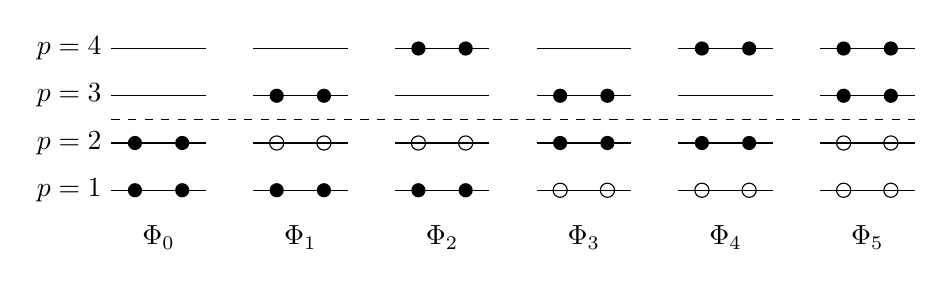
\begin{tikzpicture}[scale=0.6]
        % Draw lines
        \foreach \x in {0,3,6,9,12,15} {
            \foreach \y in {1,2,3,4} {
                \draw (\x, \y) -- (\x+2, \y);
            }
        }
        % Draw additional dashed lines
        \draw[dashed] (0, 2.5) -- (17, 2.5);

        % Labels on the left
        \foreach \y/\label in {1/$p=1$, 2/$p=2$, 3/$p=3$, 4/$p=4$} {
            \node[left] at (0, \y) {\label};
        }

        % Groundstate
        \foreach \x/\y in {0.5/1, 0.5/2, 1.5/1, 1.5/2} {
            \fill (\x, \y) circle (0.15);
        }
        \node at (1, 0) {$\ket{\Phi_0}$};

        % Phi_1
        \foreach \x in {3.5, 4.5} {
            \foreach \y in {1, 3} {
                \fill (\x, \y) circle (0.15);
            }
            \draw (\x, 2) circle (0.15);
        }
        \node at (4, 0) {$\ket{\Phi_1}$};

        % Phi_2
        \foreach \x in {6.5, 7.5} {
            \foreach \y in {1, 4} {
                \fill (\x, \y) circle (0.15);
            }
            \draw (\x, 2) circle (0.15);
        }
        \node at (7, 0) {$\ket{\Phi_2}$};

        % Phi_3
        \foreach \x in {9.5, 10.5} {
            \foreach \y in {2, 3} {
                \fill (\x, \y) circle (0.15);
            }
            \foreach \y in {1} {
                \draw (\x, \y) circle (0.15);
            }
        }
        \node at (10, 0) {$\ket{\Phi_3}$};

        % Phi_4
        \foreach \x in {12.5, 13.5} {
            \foreach \y in {2, 4} {
                \fill (\x, \y) circle (0.15);
            }
            \foreach \y in {1} {
                \draw (\x, \y) circle (0.15);
            }
        }
        \node at (13, 0) {$\ket{\Phi_4}$};

        % Phi_5
        \foreach \x in {15.5, 16.5} {
            \foreach \y in {3, 4} {
                \fill (\x, \y) circle (0.15);
            }
            \foreach \y in {1, 2} {
                \draw (\x, \y) circle (0.15);
            }
        }
        \node at (16, 0) {$\ket{\Phi_5}$};

    \end{tikzpicture}
    \caption{
        Schematic representation of the six possible Slater determinants for a system with four particles, under the constraint of no broken pairs, total spin $S = 0$, considering only the four lowest levels $p = 1, 2, 3, 4$.\label{fig:SDs}
    }
\end{figure}

Setting up the Slater determinants in second quantization, we set the ground state to be
\begin{equation*}
    \ket{\Phi_0} = a_{1+}^\dagger a_{1-}^\dagger a_{2+}^\dagger a_{2-}^\dagger \ket{0}.
\end{equation*}
We define the other Slater determinants relative to the ground state:
\begin{align*}
    \ket{\Phi_1} &= a_{3+}^\dagger a_{3-}^\dagger a_{2-} a_{2+} \ket{\Phi_0}, \\
    \ket{\Phi_2} &= a_{4+}^\dagger a_{4-}^\dagger a_{2-} a_{2+} \ket{\Phi_0}, \\
    \ket{\Phi_3} &= a_{3+}^\dagger a_{3-}^\dagger a_{1-} a_{1+} \ket{\Phi_0}, \\
    \ket{\Phi_4} &= a_{4+}^\dagger a_{4-}^\dagger a_{1-} a_{1+} \ket{\Phi_0}, \\
    \ket{\Phi_5} &= a_{4+}^\dagger a_{4-}^\dagger a_{3+}^\dagger a_{3-}^\dagger a_{2-} a_{2+} a_{1-} a_{1+} \ket{\Phi_0}.
\end{align*}

Setting up the Hamiltonian matrix in Python, we find
\begin{equation*}
    \begin{bmatrix}
        2 - g & - \frac{g}{2} & - \frac{g}{2} & - \frac{g}{2} & - \frac{g}{2} & 0 \\
        - \frac{g}{2} & 4 - g & - \frac{g}{2} & - \frac{g}{2} & 0 & - \frac{g}{2} \\
        - \frac{g}{2} & - \frac{g}{2} & 6 - g & 0 & - \frac{g}{2} & - \frac{g}{2} \\
        - \frac{g}{2} & - \frac{g}{2} & 0 & 6 - g & - \frac{g}{2} & - \frac{g}{2} \\
        - \frac{g}{2} & 0 & - \frac{g}{2} & - \frac{g}{2} & 8 - g & - \frac{g}{2} \\
        0 & - \frac{g}{2} & - \frac{g}{2} & - \frac{g}{2} & - \frac{g}{2} & 10 - g
    \end{bmatrix}
\end{equation*}

Plotted as a function of $g$, the ground state energy is shown in Fig.~\ref{fig:groundstate}.

\begin{figure}[htbp]
    \centering
    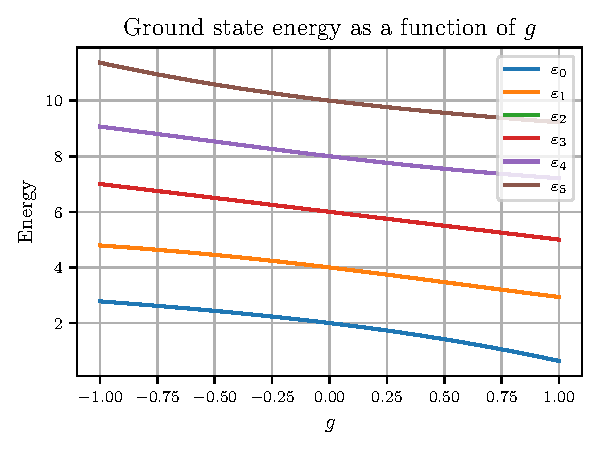
\includegraphics[width=0.8\textwidth]{figures/ground_state_energy.pdf}
    \caption{
        Ground state energy as a function of $g$ for the four-particle system with no broken pairs and total spin $S = 0$.
        The energy is given in units of the unperturbed ground state energy.\label{fig:groundstate}
    }
\end{figure}
